\documentclass[11pt,a4paper]{article}
\usepackage[utf8]{inputenc}\usepackage[T1]{fontenc}
\usepackage[margin=1in]{geometry}
\usepackage{amsmath,amssymb,booktabs,graphicx,enumitem,xcolor,parskip,titlesec}
\usepackage[hidelinks]{hyperref}
\graphicspath{{figures/}}
\definecolor{qnavy}{RGB}{20,40,75}\definecolor{qgrey}{RGB}{90,90,90}\definecolor{qred}{RGB}{150,30,30}
\titleformat{\section}{\large\bfseries\color{qnavy}}{\thesection}{0.6em}{}
\begin{document}\thispagestyle{empty}
\noindent
{\large\bfseries\color{qnavy} Report R08 --- The Lung Chromatin Arm, With Methylation}\\[2pt]
{\color{qgrey}TCGA-LUAD + LUSC, 450k arrays, 841 tumours and 74 normals. A real methylation
phenotype, and no prognostic value.}\\[6pt]
{\color{qgrey}\rule{\textwidth}{0.4pt}}

\medskip
\noindent 7 August 2026 \quad\textbullet\quad Quantara

\section*{Summary}

R06 established that KEAP1 and SMARCA4 mutations are prognostic in NSCLC using mutation data
alone, and flagged the methylation layer as the funded extension. This report delivers it:
919 open-access Illumina 450k files acquired from GDC, MD5-verified, and assembled into a
single 486{,}427 $\times$ 919 matrix.

Two findings, pointing in opposite directions.

\textbf{KEAP1 mutation carries a genuine methylation phenotype.} Within lung adenocarcinoma,
\textbf{29.4\%} of 20{,}000 tested probes are differentially methylated by KEAP1 status
(minimum $q = 1.7\times10^{-20}$), and SMARCA4 reaches 11.3\%. These survive the confounding
check that killed the third gene.

\textbf{Methylation carries no prognostic information beyond what is already free.} A
cross-validated methylation signature reaches C-index \textbf{0.486} (95\% CI 0.450--0.523) ---
no better than chance --- and adding it to a model of mutation status, stage, age and histology
moves the C-index from 0.606 to 0.602 (likelihood-ratio $p = 0.85$). Unlike R07, this is an
\emph{informative} null: with 313 events the analysis excludes any signature above C-index
0.552.

All four pre-registered positive controls fired, including the one R07 could not power:
smokers show significantly lower AHRR \texttt{cg05575921} methylation ($p = 0.0056$), confirming
in a properly powered cohort the direction R07 could only observe.

\textbf{One claim was withdrawn by the audit.} Pooled across both histologies, KMT2D looked like
the strongest hit after KEAP1 (20.7\% of probes). Within each histology separately it is
\textbf{0.0\%} in LUAD and 0.03\% in LUSC. The entire signal was the LUAD-versus-LUSC contrast
--- see \S3.

\section{Acquisition}

\begin{center}
\begin{tabular}{@{}lr@{}}
\toprule
Files downloaded and MD5-verified & 919 / 919 \\
Probes per file (identical vector, SHA-256 verified) & 486{,}427 \\
Primary tumours / solid-tissue normals & 841 / 74 \\
Technical replicates resolved (lowest \texttt{file\_id} kept) & 4 \\
Matrix NA fraction (SeSAMe masks unreliable probes) & 14.76\% \\
Probes surviving the $\leq$5\% NA filter & 392{,}489 \\
Samples matched to a clinical record & 900 / 915 \\
\bottomrule
\end{tabular}
\end{center}

Only the 450k platform was used. The same GDC query also returns 311 HumanMethylation27 and 53
EPIC~v2 files, which were \textbf{excluded before download}: mixing array generations would
confound every comparison in this report. Acquisition ran on a transient VM with a
Google-enforced one-hour cap and \texttt{DELETE} on expiry; it completed in five minutes and
the instance was then deleted explicitly and verified gone. Raw files were parsed and discarded
on the VM, so only the assembled matrix left it. GDC is a permanent archive keyed by
\texttt{file\_id}, and \texttt{evidence/MANIFEST\_450k.tsv} carries all 919 ids with MD5s, so
the raw data is re-acquirable without us storing 11.23~GiB of it.

\section{Positive controls}

\begin{center}
\begin{tabular}{@{}llll@{}}
\toprule
\textbf{Control} & \textbf{Prediction} & \textbf{Observed} & \textbf{Verdict} \\
\midrule
PC1 tumour vs normal & thousands differential & 16{,}609 / 20{,}000 probes at $q<0.05$ & holds \\
PC2 sex & near-perfect separation & \texttt{cg12026625}, AUROC 0.9994 & holds \\
PC3 AHRR \texttt{cg05575921} & lower in smokers & 0.661 vs 0.717, $p = 0.0056$ & \textbf{holds} \\
PC4 LUAD vs LUSC & separable & best probe AUROC 0.955 & holds \\
\bottomrule
\end{tabular}
\end{center}

PC1 and PC2 were the gating pair, because they test assembly and join correctness rather than
biology: PC1 fails if the matrix is scrambled, PC2 fails if samples are joined to the wrong
patients. PC2 is the same check that R07 needed to rule out a silent column-order error.

PC3 deserves its own note. R07 could only show the correct \emph{direction} at $p=0.093$,
because that cohort had 24 smokers. Here, with 220 current smokers against 81 lifelong
never-smokers, the same probe gives $p = 0.0056$ in the same direction. R07's control was
underpowered, not wrong.

\begin{center}
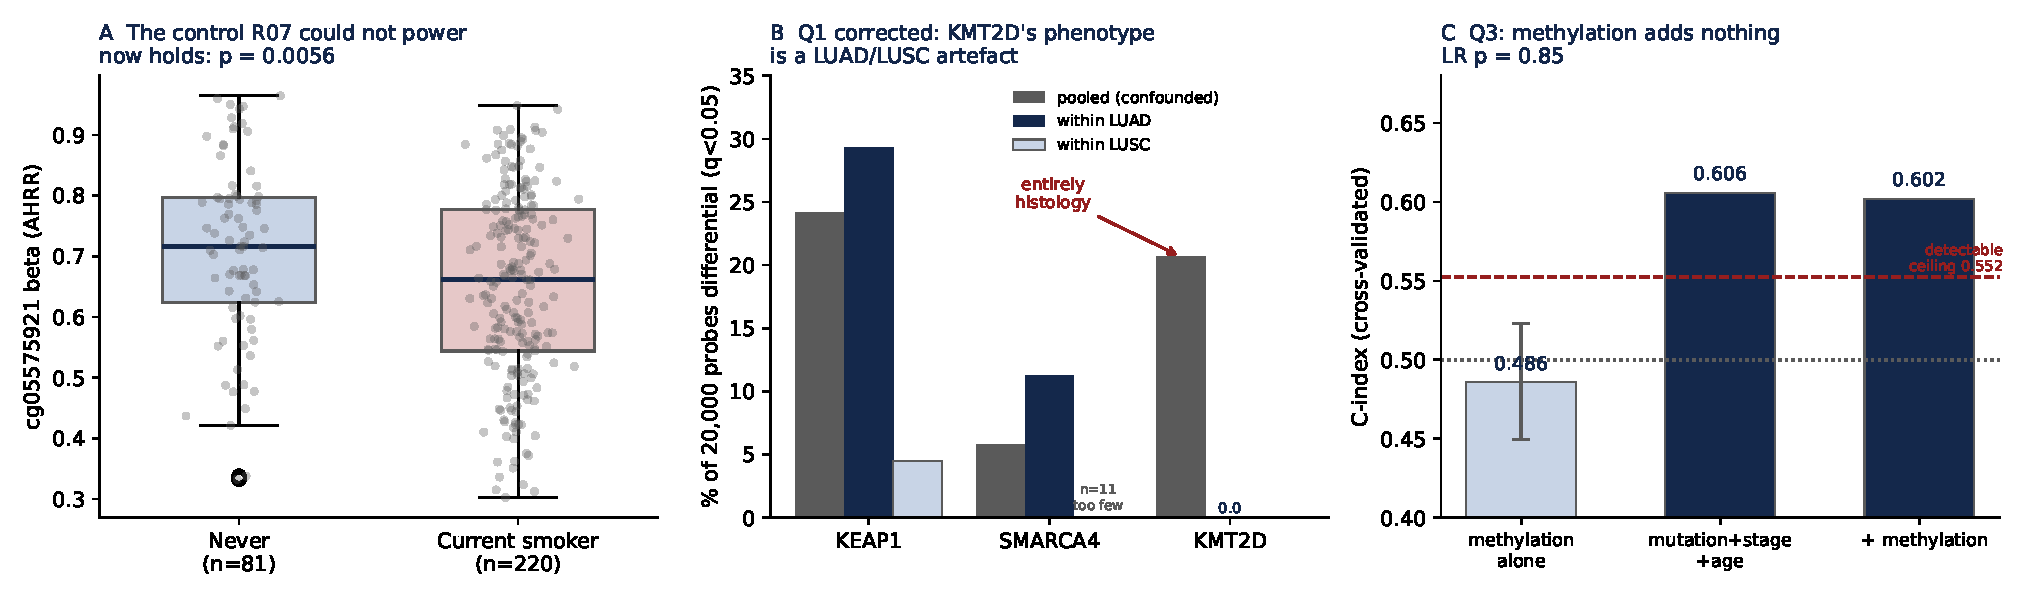
\includegraphics[width=\textwidth]{r08_panels.pdf}
\end{center}
\noindent{\small\color{qgrey}\textbf{A} The AHRR smoking control, now properly powered.
\textbf{B} Q1 before and after stratifying by histology: KEAP1 and SMARCA4 survive, KMT2D does
not. \textbf{C} Methylation alone is at chance; adding it to the clinical/mutation model
changes nothing. The dashed line is the largest C-index this cohort could have missed.}

\section{Q1 --- differential methylation by chromatin-regulator mutation}

\begin{center}
\begin{tabular}{@{}lrrrr@{}}
\toprule
\textbf{Gene} & \textbf{Mutated} & \textbf{Pooled \% sig} & \textbf{Within LUAD} &
\textbf{Within LUSC} \\
\midrule
KEAP1   & 117 & 24.2\% & \textbf{29.4\%} ($n{=}84$) & 4.5\% ($n{=}33$) \\
SMARCA4 & \phantom{0}52 & \phantom{0}5.8\% & \textbf{11.3\%} ($n{=}41$) &
  --- ($n{=}11$, too few) \\
KMT2D   & 111 & 20.7\% & \textbf{0.0\%} ($n{=}33$) & 0.03\% ($n{=}78$) \\
\bottomrule
\end{tabular}
\end{center}

\noindent{\small Percentages are of 20{,}000 randomly sampled probes reaching $q<0.05$
(Benjamini--Hochberg) on a Mann--Whitney test of mutated versus wild-type tumours.}

\textbf{The pooled column is not trustworthy, and the audit is why.} PC4 established that LUAD
and LUSC are almost perfectly separable from methylation, and mutation frequencies differ
sharply between them: KEAP1 is mutated in 17.8\% of LUAD versus 8.9\% of LUSC
($p = 1.9\times10^{-4}$), while KMT2D runs the other way at 7.0\% versus 21.1\%
($p = 2.5\times10^{-9}$). Any pooled comparison by mutation status therefore partly measures
histology.

Stratifying separates the two cases cleanly. KEAP1's signal \emph{strengthens} within LUAD
(29.4\% against 24.2\% pooled), which is what a real effect looks like once a diluting
confounder is removed. KMT2D's signal disappears entirely --- 0.0\% within LUAD, 0.03\% within
LUSC --- so all 20.7\% was the histology contrast. This is the same failure mode as R04, where
a molecular panel appeared to beat imaging until grade mix was controlled.

\section{Q2 and Q3 --- prognostic value}

\begin{center}
\begin{tabular}{@{}lr@{}}
\toprule
Tumours with usable survival (TCGA-CDR) & 811 (316 events) \\
In the Cox models, after dropping missing age & 796 (313 events) \\
\midrule
Q2 methylation signature alone, C-index & 0.486 \quad 95\% CI 0.450--0.523 \\
Q3 mutation + stage + age + histology & 0.606 \\
Q3 the same, plus methylation & 0.602 \\
Likelihood-ratio test for adding methylation & $\chi^2 = 0.03$, $p = 0.85$ \\
Minimum detectable C-index at 80\% power & 0.552 \\
\bottomrule
\end{tabular}
\end{center}

Probe selection and hyperparameters were fitted strictly inside training folds. The signature
is at chance, and the increment is nil by every measure --- C-index, likelihood ratio, and the
Cox coefficient itself (HR 1.011, $p = 0.853$). The audit re-derived Q3 under eight
cross-validation seeds and the combined model stayed at C-index 0.586--0.609, so this is not a
split artefact of the kind that changed R05's conclusion.

\textbf{This null is informative, and that distinguishes it from R07.} R07 could not detect
anything below AUROC 0.685, so its null was uninformative. Here the interval excludes any
methylation signature better than C-index 0.552. A clinically useful prognostic signature would
have to be weaker than that to have escaped detection.

\textbf{A finding for R09.} In this model KEAP1 carries HR 1.085 ($p = 0.61$) and SMARCA4
HR 1.45 ($p = 0.079$), against R06's KEAP1 HR 2.07 in the MSK circulating-tumour-DNA cohort.
This report is not the right test of that discrepancy --- its Cox model is adjusted for stage
and histology, and TCGA is predominantly resected early-stage disease whereas the MSK cohort
was advanced. R09 tests it directly, using R06's own unadjusted model and its positive controls.

\section{Audit findings}

Recorded in \texttt{evidence/audit\_addendum.json}; full reasoning in \texttt{AUDIT.md}.

\textbf{5.1 KMT2D withdrawn (\S3).} Pooled 20.7\% $\rightarrow$ 0.0\% within LUAD. Entirely
histology.

\textbf{5.2 A parsing bug crashed the first run, which was the good outcome.} The stage
covariate was parsed case-sensitively (\texttt{"Stage "}) while cBioPortal writes
\texttt{"STAGE IIIA"}, so it silently became constant and the Cox design went singular. Because
it crashed rather than fitting a degenerate model, it could not pass unnoticed --- but relying
on that is not a control, so gates \texttt{G8} (late-stage fraction must fall in 0.20--0.60;
observed 0.480) and \texttt{G9} (each covariate must be non-constant) were added. The crashed
run is retained at \texttt{evidence/gates\_FIRST\_CRASHED\_RUN.json}.

\textbf{5.3 Smoking cannot be disentangled from KEAP1 mutation, and is stated as a limitation.}
KEAP1 mutation is associated with ever-smoking (OR 3.40, $p = 0.011$), and smoking alters
methylation (PC3). Stratifying is impossible: only 4 of 81 never-smokers carry a KEAP1
mutation. So the within-LUAD KEAP1 methylation phenotype is reported as real but
\emph{not} established as independent of smoking. Its size (29.4\% of probes) makes it unlikely
to be wholly a smoking effect, but this report cannot prove that.

\section{What this settles for the lung arm}

\begin{itemize}[leftmargin=1.2em,itemsep=2pt]
\item \textbf{The methylation extension is complete, and its answer is negative for prognosis.}
Methylation adds nothing to mutation, stage and age. Further methylation acquisition for
prognostic modelling in NSCLC is not worth funding on this evidence.
\item \textbf{KEAP1 has a genuine, large methylation phenotype in LUAD.} That is a
mechanistic result, not a prognostic one, and it is the part of this report worth following up
--- ideally with a cohort containing enough never-smokers to separate it from smoking.
\item \textbf{Two of three candidate genes survived scrutiny.} KMT2D did not. The pooled
analysis would have reported it as a hit.
\end{itemize}

\section{Reproducing this report}

\begin{itemize}[leftmargin=1.2em,itemsep=1pt]
\item Acquisition: \texttt{evidence/vm\_job\_r08.py}, \texttt{evidence/startup\_r08.sh},
      \texttt{evidence/MANIFEST\_450k.tsv} (919 file ids + MD5s)
\item Analysis: \texttt{evidence/m8\_tcga\_methylation.py}; audit:
      \texttt{evidence/audit\_m8.py}
\item Config hash, written before any outcome was read:
      \texttt{07be4547c08128d0\ldots e448a240}
\item Assembled matrix: \texttt{gs://heydonto-quantara-lungcdx/data-request-2026-08/lung/}
      \texttt{tcga\_methylation\_450k/} --- \texttt{beta\_450k.npy}, \texttt{probes.txt},
      \texttt{samples.tsv}, \texttt{ACQUISITION.txt}
\item Figure: \texttt{python3 make\_figure.py}
\end{itemize}

\end{document}
